Las redes neuronales artificiales son una familia de modelos computacionales inspirados por las redes neuronales biológicas.


\begin{figure}[ht]
\centering
\begin{minipage}[b]{0.40\linewidth}
\centering
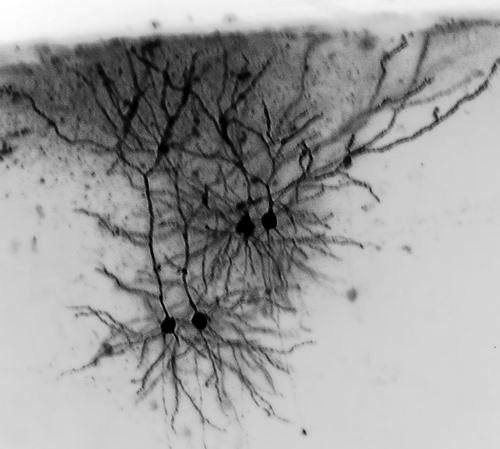
\includegraphics[width=\textwidth]{img/neuronales/biological_mouse}
\caption{Red neuronal biológica. Porción del giro cingular del cerebro de un ratón.}
\label{fig:biological}
\end{minipage}
\hspace{0.5cm}
\begin{minipage}[b]{0.40\linewidth}
\centering
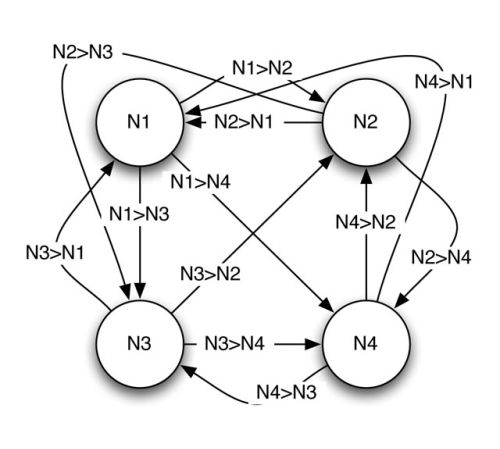
\includegraphics[width=\textwidth]{img/neuronales/artificial}
\caption{Red neuronal artificial. Los círculos representan neuronas y las flechas conexiones entre las mismas.}
\label{fig:artificial}
\end{minipage}
\end{figure}


Desde el punto de vista fisiológico, las neuronas biológicas son células que pueden estimularse eléctricamente. Las neuronas se pueden conectar unas a otras para formar \textbf{redes neuronales}, en donde se estimulan mutuamente. Los estímulos que genera una neurona son función de los estímulos actualmente recibidos, su estado interno ( generado por la historia de estímulos pasados) y el tipo y contexto (presión, alargamiento, etc) de la neurona. Los estímulos son mayormente excitativos o inhibitorios. 

Las neuronas son el componente principal del sistema nervioso, que incluye el cerebro, la médula espinal y los ganglios nerviosos periféricos. Podemos distinguir entonces tres tipos de neuronas principales, en base a la función general que cumplen:

\begin{itemize}
 \item \textbf{Sensoriales}, que responden al tacto, sonido luz y otros estímulos de los órganos sensoriales y los transmiten al cerebro y la médula espinal.
 \item \textbf{Motrices}, que reciben señales del cerebro o la médula espinal y estimulan partes del cuerpo (músculos y glándulas). 
 \item \textbf{Interneuronas} que conectan unas neuronas con otras en la misma región del cerebro o la médula espinal.
\end{itemize}


\image{neuronales/inputoutput}{0.2}{Relación entre las neuronas sensoriales, interneuronas y motrices (TODO)}

 
Desde el punto de vista histológico, las neuronas están compuestas por el cuerpo de la célula, llamado \textbf{soma}, conectores de señales entrantes, llamadas \textbf{dendritas}, y un conector de salida llamado \textbf{axón}. Las dendritas son fibras finas  y cortas que actuan como receptores de impulsos y hay una gran cantidad en cada soma. Hay un solo axón por soma, pero luego de salir de la neurona puede bifurcarse cientos de veces para conectarse con varias dendritas de otras neuronas, y puede tener hasta 1 metro de longitud en los humanos.

\image{neuronales/histologia}{0.2}{Diagrama de las partes que componen una neurona y su interconexión }

La estimulación entre neuronas ocurre mediante señales electroquímicas, que se propagan a través de las \textbf{sinapsis}, que son conexiones especializadas con otras células donde se encuentran ramas del axón de una célula con ramas de las dendritas de otra. La sinapsis no es solamente un simple conector, ya que también modula las señales entre neuronas.

Por supuesto, hay excepciones a estas reglas: neuronas que no tienen dendritas o axón, sinapsis que conectan un axón a otro axón o una dendrita a otra dendrita, etc, pero en general siguen los patrones recién descriptos.

Si bien la histología de las neuronas se estudia hace tiempo y se conoce con bastante detalle, desde el punto de vista fisiológico todavía queda mucho para descubrir sobre el sistema nervioso. Hay diversos modelos sobre cómo las neuronas cómo grupo o individuos representan y procesan información, cómo influye la arquitectura de las redes en dicha función, cómo se crean y se adaptan a las necesidades del organismo o cómo influye la codificación genética en el desarrollo del cerebro; ninguno de ellos es final, en el sentido de que no existe todavía una teoría completa sobre el funcionamiento del cerebro y el sistema nervioso.

La gran mayoría de los modelos de neuronas biológicas definen su funcionamiento en términos de ecuaciones diferenciales que describen el cambio de potencial de la misma en función del tiempo y el efecto de otras neuronas, en general basados en el modelo de Huxley-Hodgkin \cite{gerstner2002,burkitt2006}. Las neuronas que modelan son analógicas, de naturaleza continua y generalmente asincrónica, y debido a que consideran el paso del tiempo utilizan el concepto de pulsos  de voltaje generados por la neurona como señal. Dichos modelos luego se extienden para redes enteras, aunque son computacionalmente demandantes, y requieren la estimación de muchos parámetros para generarse \cite{brette2007}. Además, como mencionamos antes, representan aproximaciones al funcionamiento neuronal que todavía tienen mucho por recorrer para asemejarse al comportamiento real de una red neuronal biológica. 

Entonces, si bien se han entrenado redes neuronales artificiales basadas estrictamente en modelos biológicos, en la práctica los modelos artificiales realizan ciertas simplificaciones que los hacen más amenos a la simulación computacional y más efectivos para la resolución de tareas. 

En general, los modelos de neuronas artificiales toman en cuenta la idea de neuronas de sensoriales, interneuronas y motrices que llamaremos de \textbf{entrada}, \textbf{ocultas} y de \textbf{salida}, respectivamente; esta correspondencia no es perfecta, ya que algunas neuronas realizan varias funciones, pero es útil en general. También utilizan el concepto de las neuronas y las sinapsis como moduladoras de las señales transmitidas. La mayoría abandona la representación temporal continua por una discreta donde las simulaciones se realizan paso a paso. En la simulación las neuronas actúan de forma sincrónica, o sea, en cada paso de simulación se evalúan la entrada y la salida de cada neurona. Algunas toman en cuenta el tiempo, aunque casi siempre de forma discreta. Además, son de naturaleza digital en lugar de analógica, debido a que se suelen simular con computadoras. 


A continuación, describimos un modelo general de red neuronal sincrónica, de tiempo discreto, sin recurrencias ni estado permanente. Luego, profundizamos sobre el modelo de redes neuronales \textbf{feedforward} y dos algoritmos para su entrenamiento, \textbf{backpropagation} (propagación para atrás) y \textbf{resilient backpropagation} (propagación para atrás resiliente), así como el modelo \textbf{competitivo} de redes neuronales y el algoritmo de entrenamiento de \textbf{vector quantization} (cuantización vectorial).


